% !TEX program = pdflatex
% !TEX encoding = UTF-8
% !TEX spellcheck = en_US
\documentclass[12pt]{article}

\usepackage[margin=1in]{geometry}
\usepackage{amsmath,amsthm,amssymb}
\usepackage{graphicx}
\usepackage{hyperref} % Uso de links
\usepackage[version=4]{mhchem}
\usepackage{siunitx}
\usepackage{enumerate}
% \usepackage{tcolorbox}
\usepackage{titlesec}
\usepackage{booktabs}

\titleformat{\subsection}
  {\normalfont\large\bfseries}{}{0em}{}

\setlength{\parindent}{0em}

\begin{document}

% --------------------------------------------------------------
%                         Start here
% --------------------------------------------------------------

\title{Mechanical Properties of Materials (MSAE 4215), Spring 2019\\ Homework 1 Solutions}
\author{Qi Zhang}
\date{\today}

\maketitle

\tableofcontents

\section{Problems}

\subsection{1.1}
One widely used empirical potential for the energy between two atoms with
spacing $d$ is the Morse potential, written as
\begin{equation}
	D(e^{-2\alpha(d - d_0)} - 2e^{-\alpha (d - d_0)})
\end{equation}
Sample values for \ce{Cu} are $D = 343$ meV, $\alpha = \SI{1.36}{\per\angstrom}$.
For a diatomic bond of \ce{Cu2},
\begin{enumerate}[(a)]
	\item Calculate the ``spring constant" $f$, assuming an interatomic spacing of \SI{0.209}{\nano\meter}.

	      \textbf{Solution:}
	      \begin{equation}
		      \begin{split}
			      f &= \Big( \frac{ \partial^2 U }{ \partial d^2 } \Big)_{ d = d_0 } \\
			      &= D \Big( 4 \alpha^2 e^{-2\alpha(d - d_0)} - 2 \alpha^2 e^{-\alpha(d - d_0)} \Big)_{ d = d_0 } \\
			      &= 2 \alpha^2 D \approx \SI{20.3}{\newton\per\meter} \approx \SI{1.27}{\electronvolt\per\square\angstrom}
		      \end{split}
	      \end{equation}

	\item Calculate the anharmonic coefficient $g$ and parameter $s$.

	      \textbf{Solution:}
	      \begin{equation}
		      \begin{split}
			      g &= \Big( \frac{ \partial^3 U }{ \partial d^3 } \Big)_{ d = d_0 } \\
			      &= D \Big( -8 \alpha^3 e^{-2\alpha(d - d_0)} + 2 \alpha^3 e^{-\alpha(d - d_0)} \Big) \\
			      &= -6 \alpha^3 D \approx \SI{-8.28e11}{\joule\per\cubic\meter} \approx \SI{-5.18}{\electronvolt\per\cubic\angstrom}
		      \end{split}
	      \end{equation}
	      and \begin{equation}
		      s = \frac{g}{2 f} = \SI{-2.04}{\per\angstrom}.
	      \end{equation}

	\item Calculate the coefficient of thermal expansion $\alpha$ for the bond.

	      \textbf{Solution:}
	      \begin{equation}
		      \alpha = -\frac{s k_B}{d_0 f} \approx \SI{6.6e-5}{\per\kelvin}
	      \end{equation}

	\item Estimate the ratio of elastic modulus at room temperature to that
	      at zero temperature, $E(\SI{300}{\kelvin}) / E(\SI{0}{\kelvin})$ considering one bond only.

	      \textbf{Solution:}
	      \begin{equation}
		      \frac{E(\SI{300}{\kelvin})}{E(\SI{0}{\kelvin})} = 1 - \frac{2 s^2 k_B}{f} T \approx 0.83.
	      \end{equation}

	\item For (FCC) \ce{Cu}, with lattice parameter \SI{0.36}{\nano\meter}, calculate the cohesive energy.
	      For simplicity, consider only nearest neighbor interactions ($12$ in the crystal).

	      \textbf{Solution:}
	      The distance between $2$ nearest \ce{Cu} is
	      \begin{equation}
		      d = \frac{a}{\sqrt{2}} = \SI{0.255}{\nano\meter},
	      \end{equation}
	      in a FCC crystal. So
	      \begin{equation}
		      U(d) = \frac{1}{2} \times 12 D(e^{-2\alpha(d - d_0)} - 2e^{-\alpha (d - d_0)})
		      \approx \SI{-2.59e-19}{\joule} \approx \SI{-2.05}{\electronvolt}.
	      \end{equation}
	      We devide it by $2$ because of double counting.
\end{enumerate}

\subsection{1.2}
Determine the polarization character of the optical and acoustic modes of the diatomic
lattice by backsubstituting the eigenfrequencies $\omega$ in Eq $1.39$ into the eigenvalue
Equation $1.34$, and solving for $A$ and $B$. How do the atoms move?

\textbf{Solution:}
From equation $1.34$, if $k \ll \frac{1}{a}$, we have
\begin{equation}
	\begin{cases}
		\omega_{-} \approx \omega_0 k a, & \text{acoustic mode}, \\
		\omega_{+} \approx 2 \omega_0,   & \text{optical mode},
	\end{cases}
\end{equation}
and $\cos (k a) \approx 1 - \frac{k^2 a^2}{2}$.
Equation $1.39$ is from the limit of equal masses, i.e., $\eta = 1$, backsubstitute it into equation $1.34$,
for the acoustic mode,
\begin{equation}
	\begin{bmatrix}
		1 - \frac{k^2 a^2}{2}  & -1 + \frac{k^2 a^2}{2} \\
		-1 + \frac{k^2 a^2}{2} & 1 - \frac{k^2 a^2}{2}
	\end{bmatrix}
	\begin{bmatrix}
		A \\
		B
	\end{bmatrix} = 0,
\end{equation}
then we have $A = B$. So the atoms move in the same direction and amplitude.
For the optical mode,
\begin{equation}
	\begin{bmatrix}
		-1                     & -1 + \frac{k^2 a^2}{2} \\
		-1 + \frac{k^2 a^2}{2} & -1
	\end{bmatrix}
	\begin{bmatrix}
		A \\
		B
	\end{bmatrix} = 0,
\end{equation}
then we have $A = -B$, so the atoms move in the opposite direction but with the same amplitude.

\subsection{1.3}

Derive the dispersion relation for a monatomic lattice: $A$ atoms only,
separated by a lattice spacing of $a$, with spring constant $k$.
Using the Bloch theorem, show (graphically) that the result is
identical to that for the diatomic lattice with $m_A = m_B$ shown in figure $1.3$.
\textit{Hint:} the first Brillouin zone boundary for a lattice with lattice parameter
$2a$ is at half the value of that for a lattice with lattice parameter $a$,
and the reduced representation for one is in the extended representation for the other.

\textbf{Solution:}
For a 1D monatomic lattice, the equation of motion for the $n$th atom,
considering only the nearest neighbor interactions, is:
\begin{equation}
	m \ddot{A}_n = -k_A (2A_n - A_{n-1} - A_{n+1}).
\end{equation}
Consider wavelike solution for $n$th atom,
\begin{equation}
	A_{n} = A e^{i (k x_n - \omega t)},
\end{equation}
where $x_n = n a$, we get
\begin{align}
	-m \omega^2 A e^{i (k n a - \omega t)} & = -k_A A(2 e^{i (k n a - \omega t)} - e^{i (k (n-1)a - \omega t)} - e^{i (k (n+1)a - \omega t)}), \\
	m \omega^2 A e^{i k n a}               & = k_A A(2 e^{i k n a} - e^{i k (n-1)a} - e^{i k (n+1)a}),                                         \\
	m \omega^2                             & = k_A (2 - e^{-i k a} - e^{i k a}),                                                               \\
	m \omega^2                             & = k_A (2 - 2 \cos(k a)),                                                                          \\
	\omega^2                               & = 2 \omega_0^2 (1 - \cos(k a)),                                                                   \\
	\omega                                 & = 2 \omega_0 \bigg| \sin \frac{k a}{2} \bigg|,
\end{align}
since
\begin{equation}
	\bigg| \sin \frac{x}{2} \bigg| = \sqrt{\frac{1 - \cos x}{2}}.
\end{equation}
Plotting this extended dispersion relation in figure \ref{fig:monatomic}, for the 1D monatomic lattice, the diatomic lattice, and the first
Brillouin zone boundaries for the monatomic lattice and diatomic lattice we can verify that the extended
representation for the diatomic lattice ``contains” that of the monatomic lattice when
$m_A = m_B$. In this range, they are identical.
Note: the extended representation of the diatomic lattice includes both the solid green line and
the dotted blue line.
\begin{figure}[h]
	\centering
	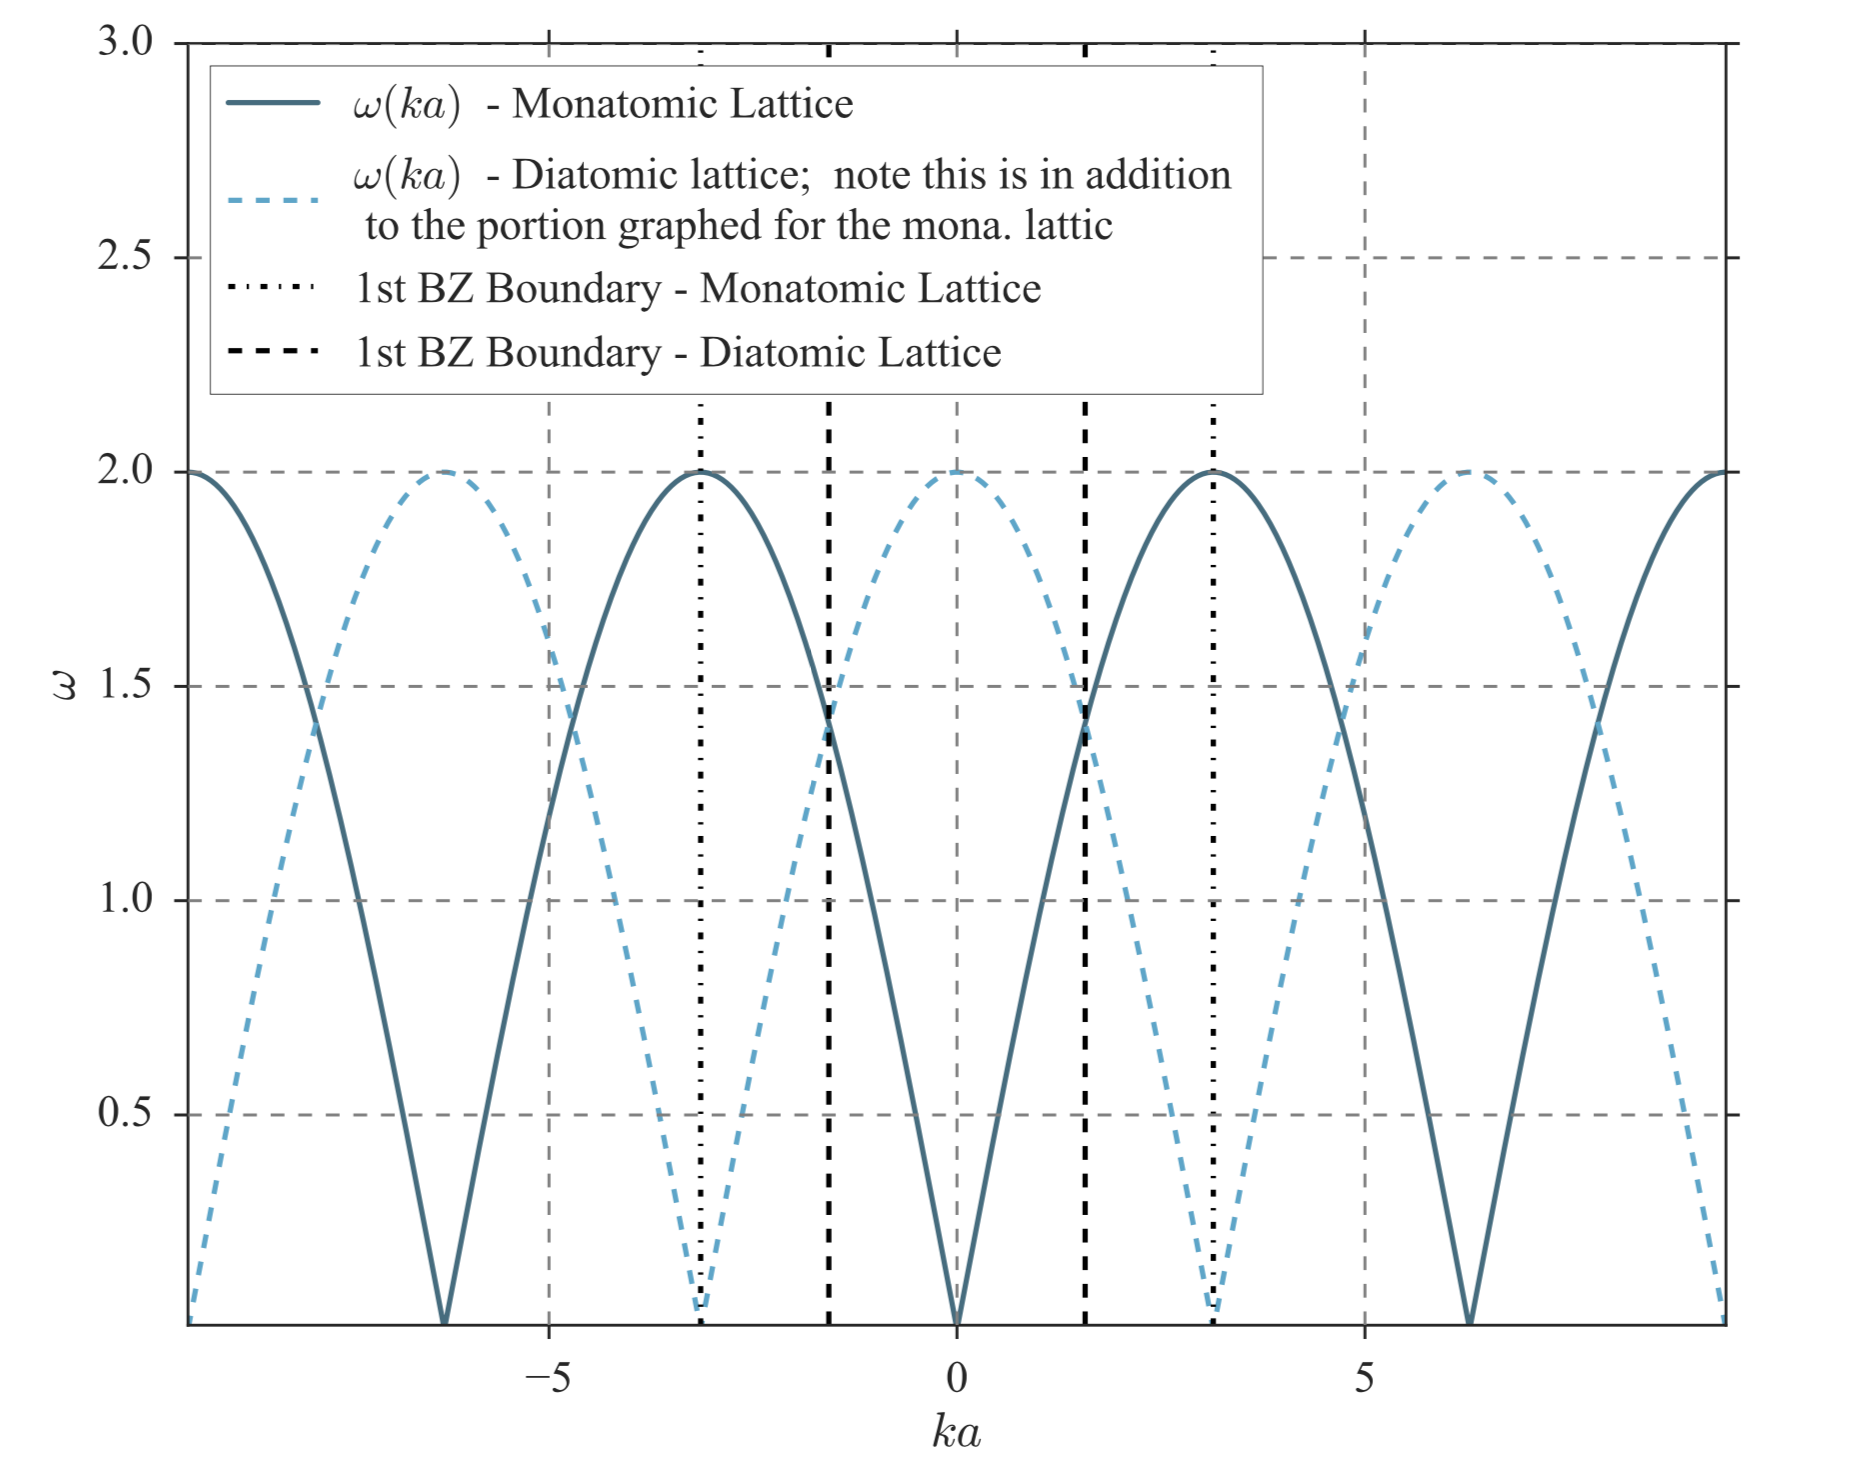
\includegraphics[width=0.8\linewidth]{images/1_3.png}
	\caption{Extended dispersion relation for 1D diatomic and monatomic lattices, credit to Michael Carter.}
	\label{fig:monatomic}
\end{figure}

\subsection{1.4}
Will there be a relationship between cohesive energy and the Debye temperature,
according to the power law model for potentials?
Assume two scenarios: one where the $A$ and $B$ coefficients change by a
common factor, and one where they do not. What do you expect? Make a
table of cohesive energies (in \si{\electronvolt}/atom) and Debye temperatures $\theta$ (in
\si{\kelvin}) for \ce{Si}, \ce{Ge}, \ce{Sn}, \ce{Cu}, \ce{Ag}, \ce{Au} and rationalize your results.

\textbf{Solution:}
First lets consider how the the Debye temperature changes when $A$ and $B$ change by a constant factor k. The
Debye temperature is:
\begin{equation}
	\theta = \frac{\hbar v_m}{k_B} (6 \pi^2 n_\text{at})^\frac{1}{3},
\end{equation}
Thus $\theta \propto v_m n_\text{at}^\frac{1}{3}$.
And, using the Debye approximation $v_m = \omega_0 a$ with $n_\text{at} \propto (1/a^3)^\frac{1}{3}$, then
\begin{equation}
	\theta \propto \omega_0.
\end{equation}
The resonance frequency is $\omega_0 \equiv \sqrt{f / m}$, then
\begin{equation}
	\theta \propto \sqrt{f},
\end{equation}
where
\begin{equation}
	f = \Big( \frac{ \partial^2 U }{ \partial d^2 } \Big)_{ d = d_0 }
	= -2 A d_0^{-3} + n (n + 1) B d_0^{-n - 2}.
\end{equation}
If $A$ and $B$ change by a constant factor $c$, the new force constant is
\begin{equation}
	f' = -2 (c A)d_0^{-3} + n (n + 1) (c B) d_0^{-n - 2} = c f,
\end{equation}
so the new Debye temperature is
\begin{equation}
	\theta' \propto \sqrt{c} \theta.
\end{equation}
Now we can consider how the cohesive energy changes when $A$ and $B$ change by a constant
factor $c$. First, consider the equilibrium spacing:
\begin{equation}
	d_0' = \bigg( n\frac{c B}{c A} \bigg)^{\frac{1}{n - 1}} = \bigg( \frac{n B}{A} \bigg)^{\frac{1}{n - 1}} = d_0,
\end{equation}
this value does not change. Then cohesive energy is:
\begin{equation}
	U_0' = U(d_0) = - c A d_0^{-1} + c B d_0^{-n} = c U_0.
\end{equation}
Thus, overall we'd expected, $\theta$ to vary linearly with $\sqrt{U}$,
when $A$ and $B$ change by a constant factor $c$.


When $A$ and $B$ change by a non-constant factor $c_1$ and $c_1 c_2$:
\begin{equation}
	f' = -2 (c_1 A) d^{-3} + n(n + 1) (c_1 c_2 B) d^{-n-2} = c_1 \Big( -2 A d^{-3} + n(n+1) (c_2 B) d^{-n-2}\Big).
\end{equation}
Again we can consider the impact on the cohesive energy. First through the equilibrium spacing, which in this
case does change:
\begin{equation}
	d_0' = \bigg( n \frac{c_1 c_2 B}{c_1 A} \bigg)^{\frac{1}{n - 1}} = \bigg( n \frac{c_2 B}{A} \bigg)^{\frac{1}{n - 1}}.
\end{equation}
Then cohesive energy is:
\begin{equation}
	U_0' = U(d_0') = -(c_1 A) d_0'^{-1} + (c_1 c_2 B) d_0'^{-n}.
\end{equation}

\begin{table}[h]
  \centering
  \caption{Cohesive energy and Debye temperature for selected elements.}
    \begin{tabular}{ccc}
    	\toprule
    Element & Cohesive energy (\si{\electronvolt}/atom) & Debye temperature (K) \\
     \midrule
    \ce{Si} & 4.63  & 625 \\
    \ce{Cu} & 3.49  & 315 \\
    \ce{Ge} & 3.85  & 360 \\
    \ce{Sn} & 3.14  & 200 \\
    \ce{Ag} & 2.95  & 215 \\
    \ce{Au} & 3.81  & 170 \\
    \bottomrule
    \end{tabular}%
  \label{tab:pro14}%
\end{table}%

\textbf{In this case, all we can say is that no clear relationship exists.}
Tabulated cohesive energies, $U_0$, vs.
Debye temperatures, $\theta$, for the requested elements are listed in table 1.
Plotting $\sqrt{U_0}$ vs. $\theta$, as done in figure 2, shows a linear relationship,
except for \ce{Au}. Some additional figures are provided at the end of the solution
set to help visualize how changing the power law constants changes the $U(d)$, $d_0$, $U_0$
and $f \propto \partial^2 U / \partial^2 d$. These
are not definitive relationships for all such changes in the power law constants and are really meant only to
illustrate a few simple permutations of possible $A$ and $B$ values.
Further, these are provided in addition to the
problem solution, as a visual aid, and were not actually required as part of the HW.
\begin{figure}[h]
	\centering
	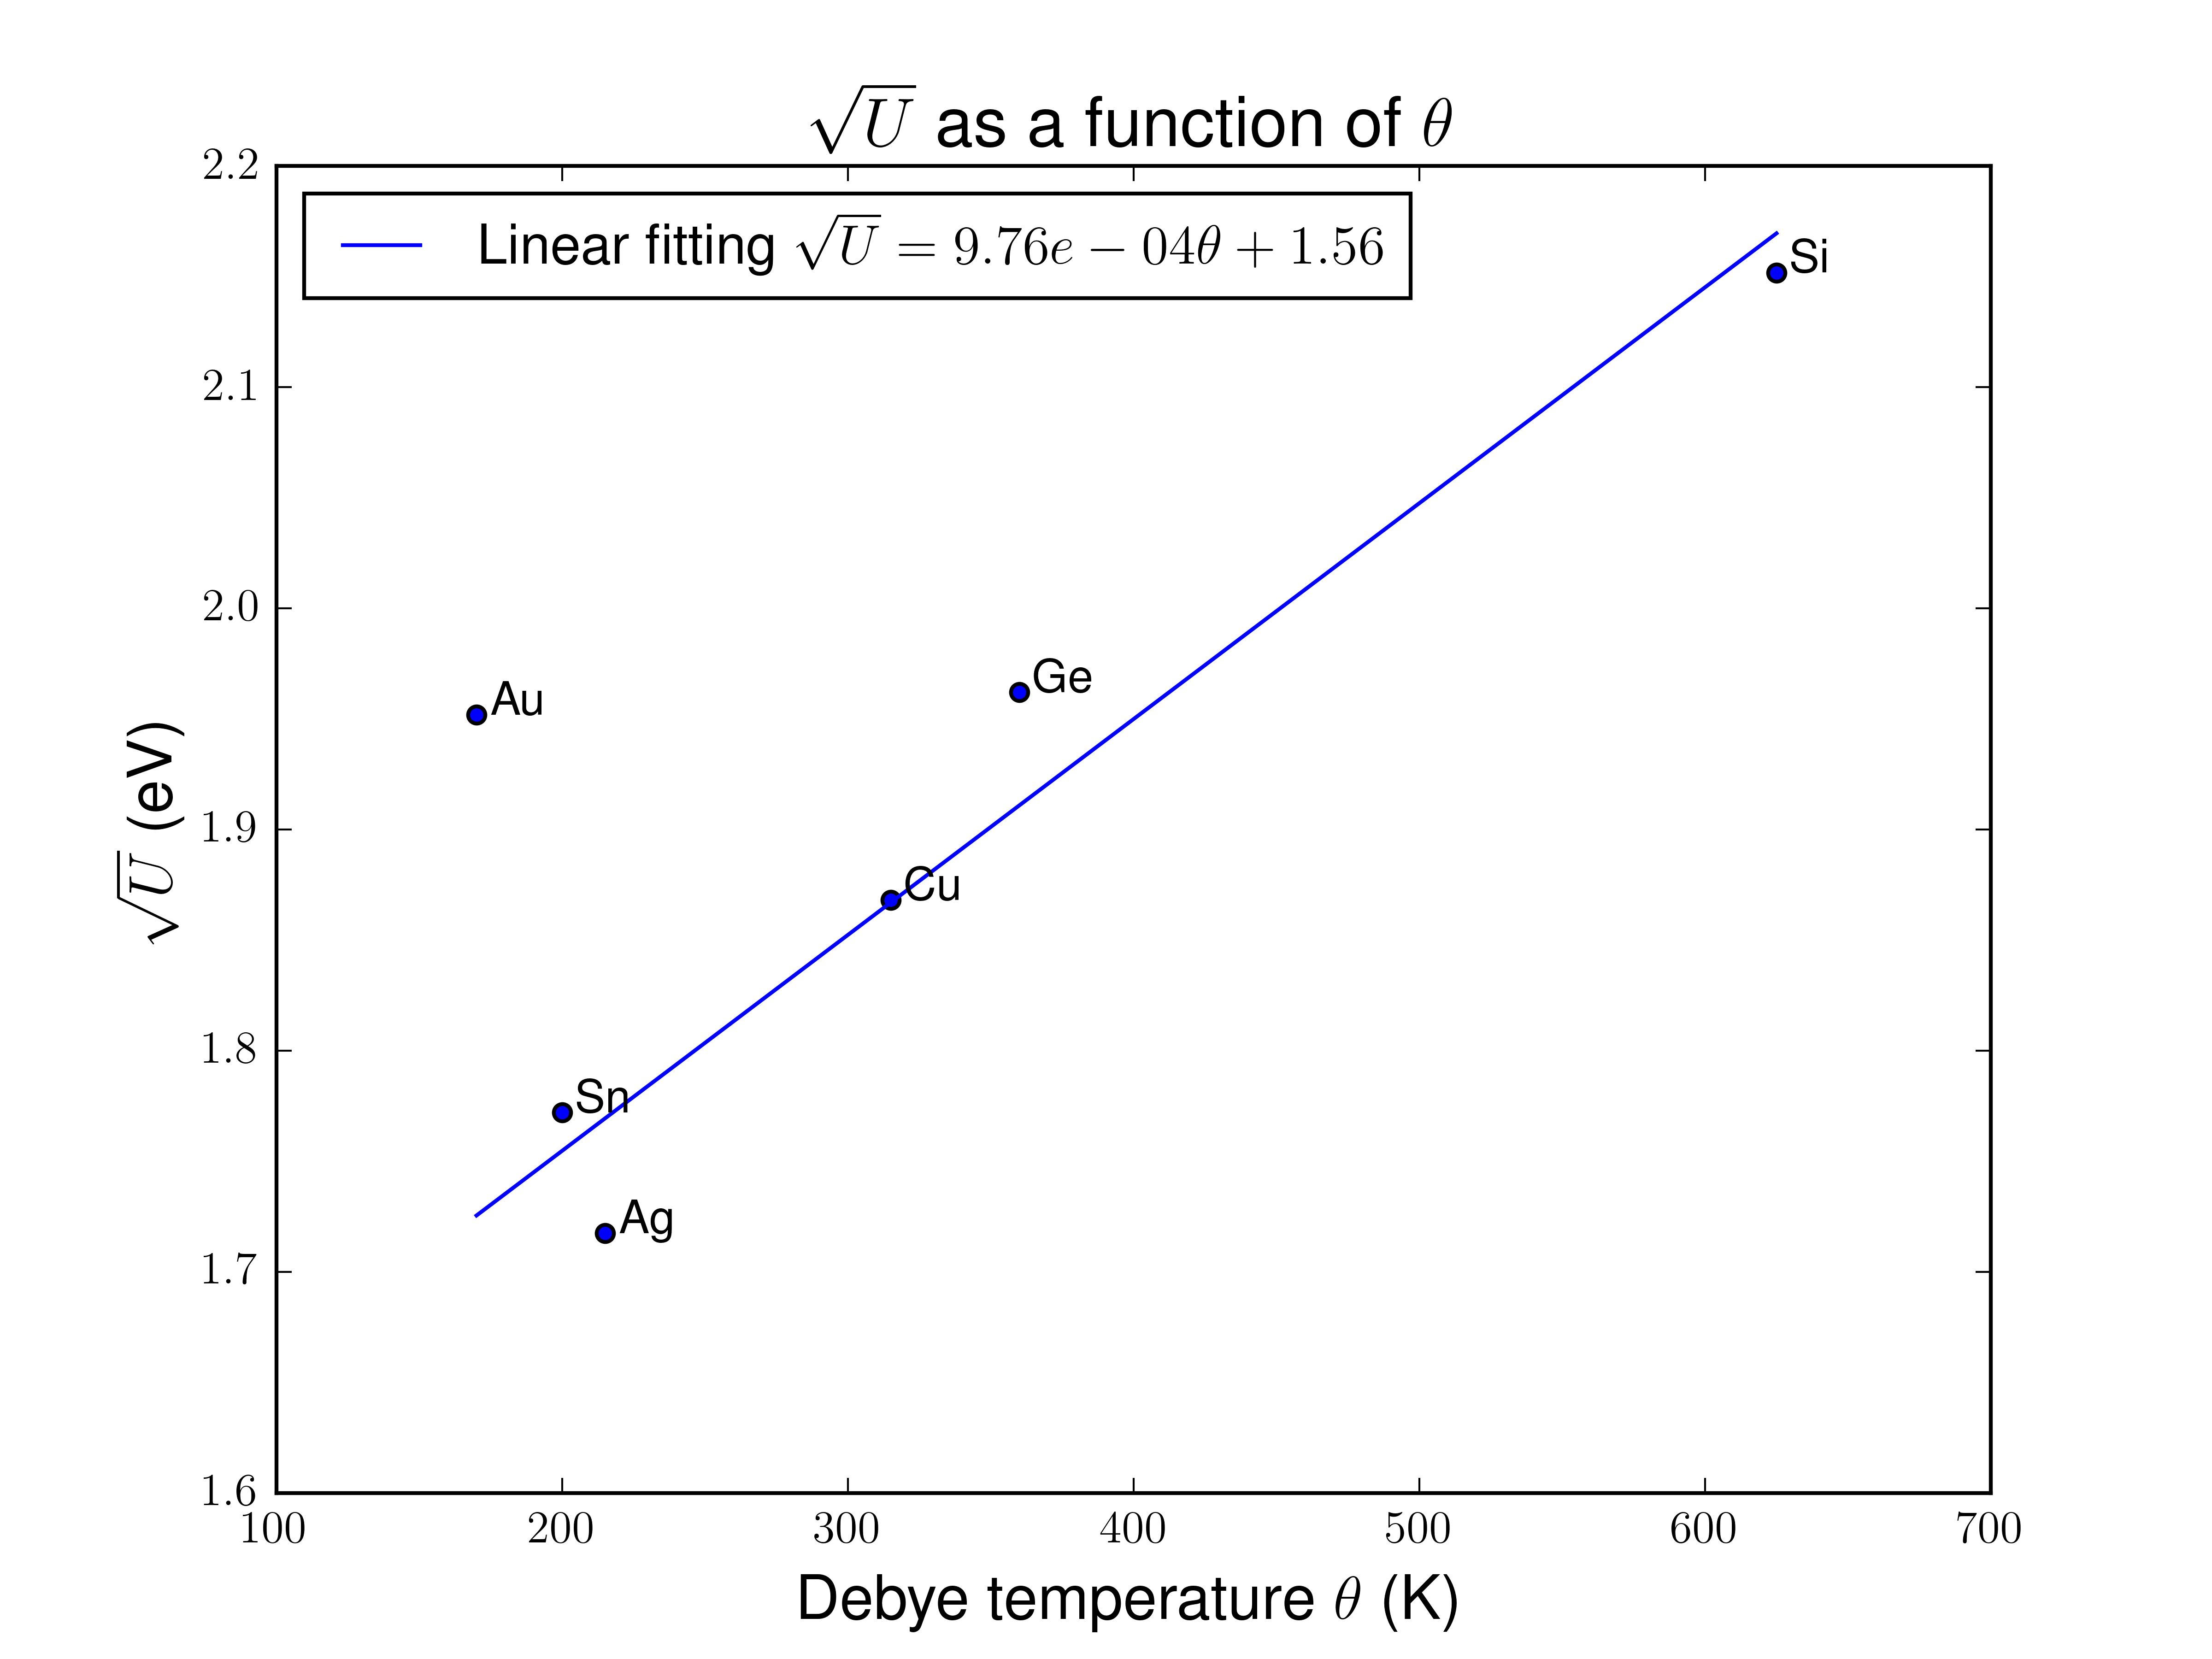
\includegraphics[width=0.8\linewidth]{images/pro_1_4}
	\caption{The square root of cohesive energy and Debye temperature for selected elements, and a linear fitting.}
	\label{fig:pro14}
\end{figure}



% --------------------------------------------------------------
%     You don't have to mess with anything below this line.
% --------------------------------------------------------------

\end{document}